\graphicspath{{Chapitre_2/Images/}}
\chapter{Introduction}\label{introduction}
\quad\, Since the end of the 17th century, people have started to study the conversion of the energy into a useful form. The purpose was to utilize the available raw energy to produce works.

Denis Papin, a french person borned in 1647 in the region of Chitenay, developed one of the first conversion machine in 1690. The machine, a steam piston engine, was powered by steam which produced a back and forth movement of the piston head generating power. 

\begin{figure}[h]
    \centering
    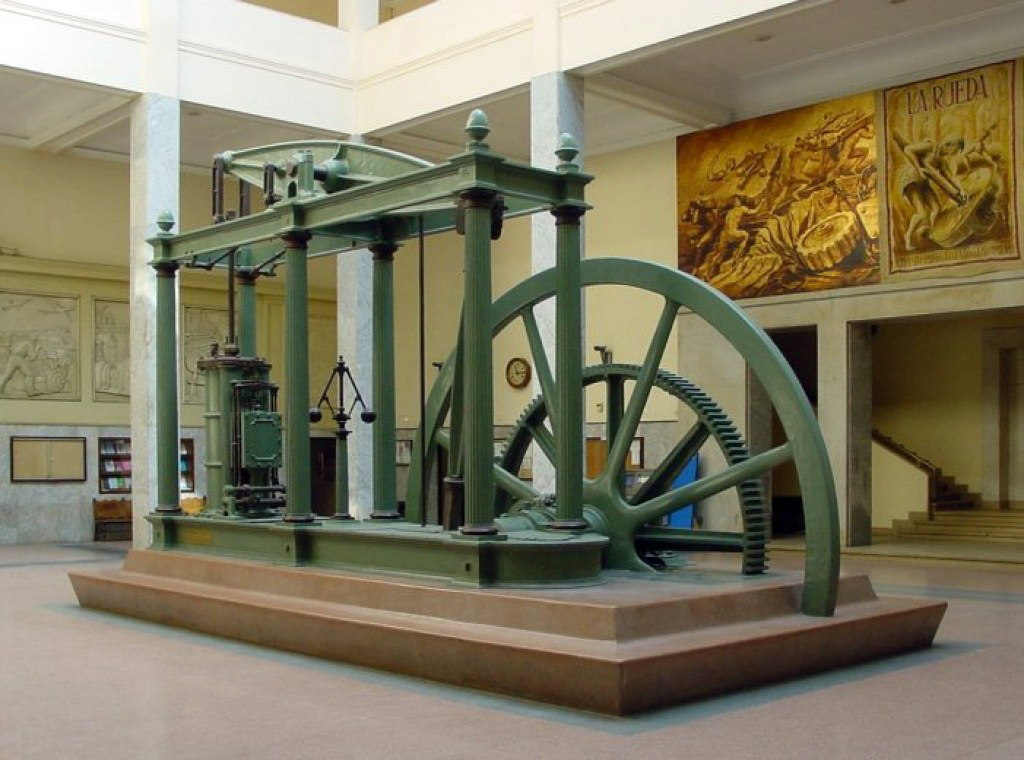
\includegraphics[width=0.6\textwidth]{Chapitre_1/Images/Maquina_vapor_Watt_ETSIIM.jpg}
    \caption{Watt steam machine\cite{Watt}}
    \label{fig:Watt}
\end{figure}

Then, later in the 18th, the British James Watt (1736 - 1819) invented and commercialized a steam machine. Thanks to the great marketing around his product, the machine was very successful among the merchants. Indeed, at this time many machines were powered by horses.\\

James Watt saw this as an opportunity by creating a unit to compare its machines to the horses. The name of the unit was the horse power. Later the power will be expressed in Watt (W) in tribute to James Watt. One of the machine built by Watt is depicted on the Figure \ref{fig:Watt}.

This progressively lead to the implementation of the steam machines in Europe, and it was one of the most important element of the industrial revolution. Indeed, aside the progressive replacement of the horses, wind and water mills also started to be replaced by mills powered by steam. A the beginning of the 19th, other fields like mining or merchandise transportation also started to utilize the steam machine technology as well.

In 1872, the American George Brayton (1830 - 1892) proposed the Brayton cycle as a ''reciprocating oil-burning engine'' \cite{Boles2006}. His engine consisted in a large cylinder where the compression, the combustion and, the expansion of the gas were successively performed. 

Nowadays, the Brayton cycle is used for gas turbines where the compression and expansion takes place in rotating machinery, also called turbomachinery. Basically, the Brayton cycle is composed of three parts. 

First the compressor that will compressor the ambient air to some pressure level. Then, there is a combustion chamber that will heat-up the air to augment its level of energy. This heating-up is performed thanks to the injection of fuel into the combustion chamber. Finally, the resulting gases from the combustion is expanded into a turbine. the power produced by the expansion is partly consumes by the compressor while the rest is used to feed any kind of power receiver. The expanded gas is then released to the atmosphere. This cycle is depicted in the Figure \ref{fig:C1_GT} where the receiver is electrical generator.

\begin{figure}[h]
    \centering
    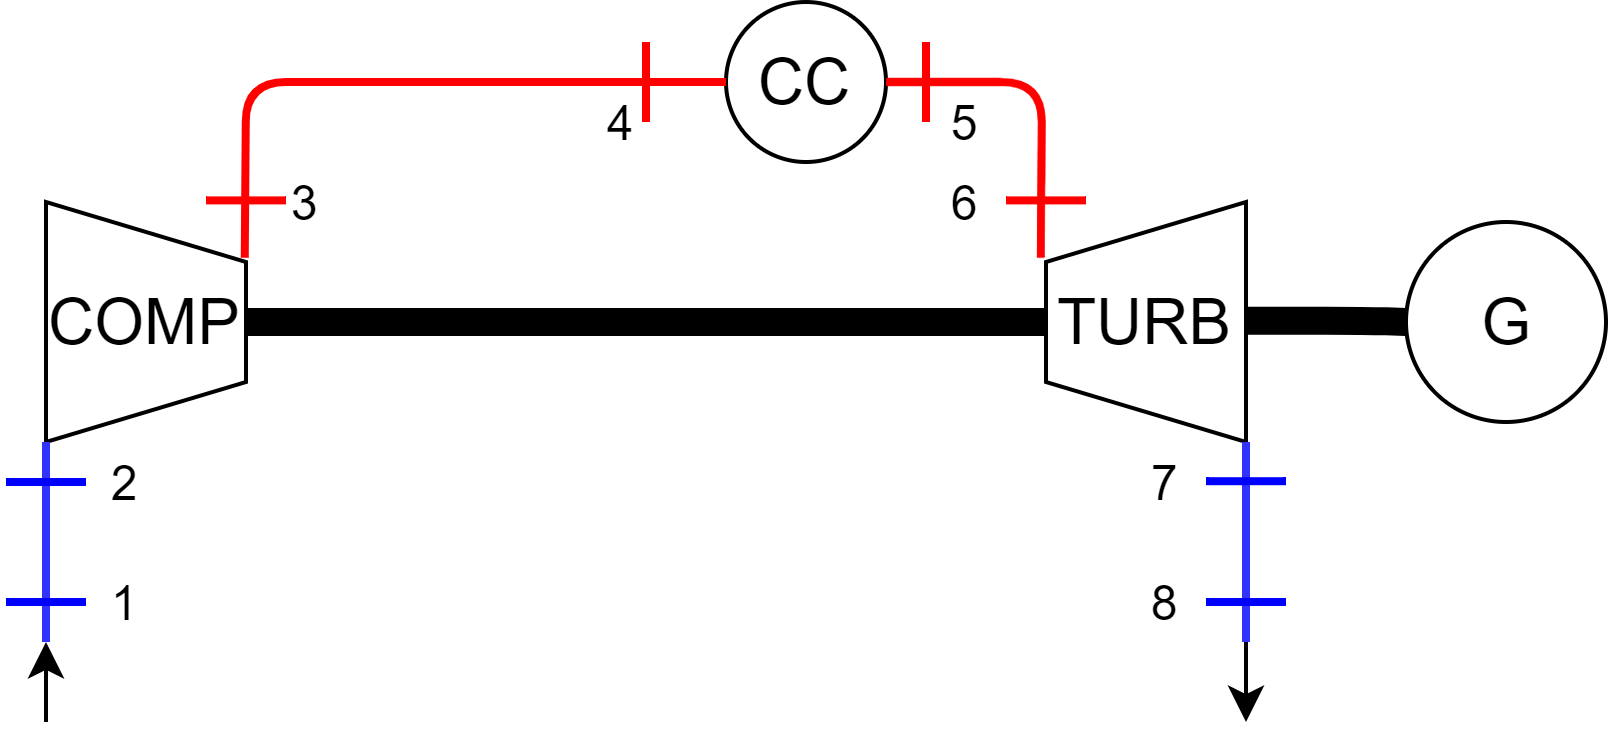
\includegraphics[width=0.6\textwidth]{Chapitre_1/Images/GT.png}
    \caption{Brayton gas cycle}
    \label{fig:C1_GT}
\end{figure}
There exists many variants of the Brayton gas cycles. The one proposed above is the most simple one where the air goes through a compressor, a combustion chamber and a turbine before returning to the environment. 

Variants are Brayton cycle where heat-exchangers are used to recover heat when it is possible, or cycles where the compression and/or the expansion are split into multiple stages, etc...

All these variants have be though to solve problems encounter and to enlarge the range of possible applications where the Brayton gas cycle can be used. For instance, Brayton cycle are used in aircraft for the propulsion, or are integrated within a power plant to produce electricity.\\

This work is focused on the improvement of a computer code that is programmed to assess the performance of a given configuration of the Brayton cycle. While some additions to the program were done to increase its modularity, the main improvements are ones that will allows the computer code the be closer from the experimental regarding the performance of the simulated Brayton cycle. \\

Not all the possible improvements will be consider for this master thesis. The main concern will be on the turbomachinery and how to simulate the influence of the operating conditions on their performances based on performance maps. These maps can be considered as the footprint of each turbomachinery.  The purpose will be to be able to easily modify the program by switching from one map to another one. Also, the integration of performance maps will give the ability to see the impact of the rotational speed of the compressor and turbine on their respective behaviors.


